\documentclass[handout, 10pt]{beamer}

%\usepackage[backend=bibtex,firstinits=true,style=verbose-inote,citestyle=authortitle]{biblatex}
\usepackage{bm}
\usepackage{graphicx}
\usepackage{subcaption}
\usepackage{amsmath}
\usepackage{amsfonts}
\usepackage{makecell}
\usepackage{filecontents}
\usepackage{biblatex}
% \newcommand{\expect}[2][]{
\ifthenelse{\equal{#1}{}}{
\mathbb{E}\left[#2\right]
}{
\underset{#1}{\mathbb{E}}\left[#2\right]
}}

\newcommand{\cov}[2][]{
\ifthenelse{\equal{#1}{}}{
\text{Cov}\left[#2\right]
}{
\underset{#1}{\text{Cov}}\left[#2\right]
}}


\newcommand{\var}[2][]{
\ifthenelse{\equal{#1}{}}{
\text{Var}[#2]
}{
\underset{#1}{\text{Var}}[#2]
}}

\newcommand{\loss}[2][]{
\ifthenelse{\equal{#1}{}}{
\mathcal{L}(#2)
}{
\mathcal{L}_{#1}(#2)
}}

\newcommand{\kl}[2]{
\text{D}_\text{KL}[#1 \parallel #2]
}

\newcommand{\R}{\mathbb{R}}
%\newcommand{\Prob}{\mathbb{P}}

\newcommand{\1}[1]{\mathds{1}\{#1\}}


%\usecolortheme{dolphin}
\setbeamertemplate{navigation symbols}{}
\setbeamertemplate{section in toc}{\inserttocsectionnumber.~\inserttocsection}

\begin{filecontents*}{references.bib}
@incollection{WANN,
title = {Weight Agnostic Neural Networks},
author = {Gaier, Adam and Ha, David},
booktitle = {Advances in Neural Information Processing Systems 32},
editor = {H. Wallach and H. Larochelle and A. Beygelzimer and F. d\textquotesingle Alch\'{e}-Buc and E. Fox and R. Garnett},
pages = {5364--5378},
year = {2019},
publisher = {Curran Associates, Inc.},
url = {http://papers.nips.cc/paper/8777-weight-agnostic-neural-networks.pdf}
}
\end{filecontents*}

\addbibresource{references.bib}


\title{Weight Agnostic Neural Networks\footnote{\citepaper{WANN}}}
%\subtitle{}
%\author{Ivan Skorokhodov}
%\date{}
%\logo{
\includegraphics[height=1cm]{images/ipavlov-logo.png}}

\newcommand{\citepaper}[1]{\citetitle{#1} by \citeauthor{#1}}

%\graphicspath{{./images}}

%\usetheme{lucid}
\begin{document}

\begin{frame}
    \titlepage
\end{frame}

\begin{frame}{Overview}
    \begin{itemize}
        \item\pause Animals and humans have a lot of innate abilities and inclinations:
            \begin{itemize}
                \item\pause A colt can walk within hours after birth
                \item\pause Turkeys can visually recognize predators shortly after hatching
                \item\pause Sharks are attracted to blood immediately after birth
                \item\pause Spiders are born ready to hunt
            \end{itemize}
        \item\pause But modern neural networks are trained from scratch on enormous datasets...
        \item\pause Authors performed NAS to find such architectures that would have good performance without any training
        \item\pause I.e. they search for architectures with a very strong inductive bias towards some task
    \end{itemize}
\end{frame}

\begin{frame}{Evolutionary algorithm overview}
    \begin{enumerate}
        \setcounter{enumi}{-1}
        \item\pause Create a population of minimal networks (linear and sparse)
        \item\pause Evaluate each network for different random weights
        \item\pause Rank by performance and complexity
        \item\pause Create a new population by varying the best models. Go to step 1.
    \end{enumerate}
\end{frame}

\begin{frame}{Stage 1 of evolution. Evaluation of networks}
\pause Authors use not just random weights, but \textit{shared} random weights (from a tiny pool of values):
\begin{itemize}
    \item\pause First, randomly sample a value from $\{-2, -1, -0.5, 0.5, 1, 2\}$.
    \item\pause Second, set each network weight to this value
    \item\pause Then compute the performance
\end{itemize}

\pause Author use 3 metrics to select best-performing models:
    \begin{itemize}
        \item\pause Mean performance: average accuracy over different random weights
        \item\pause Max performance: accuracy of the best-performing weights
        \item\pause Complexity: number of connections in the network
    \end{itemize}
\end{frame}


\begin{frame}{Stage 2 of evolution. Ranking}
\pause Instead of using hand-crafted weights sums of metrics, authors use dominance relations to detect the winners in a population:
\begin{itemize}
    \item\pause Define \textit{dominance relation}: model $f$ dominates $f'$ ($f \succ f'$) if it beats $f'$ in all the metrics.
    \item\pause For each model $f$ compute $N_f$: number of models it dominates on.
    \item\pause Sorting by $N_f$ gives us the best-performing models
    \item\pause This allows models with the least complexity to survive since no other model can dominate upon them (but if they have low performance they may die because they won't be able to dominate upon anyone either).
\end{itemize}

%Besides, since complexity payoff only in longterm they do not evaluate based on mean performance and complexity in 80\% of cases and on max performance and complexity in other 20\% of cases.
\end{frame}

\begin{frame}{Stage 3 of evolution. Mutating models}
\begin{figure}
    \centering
    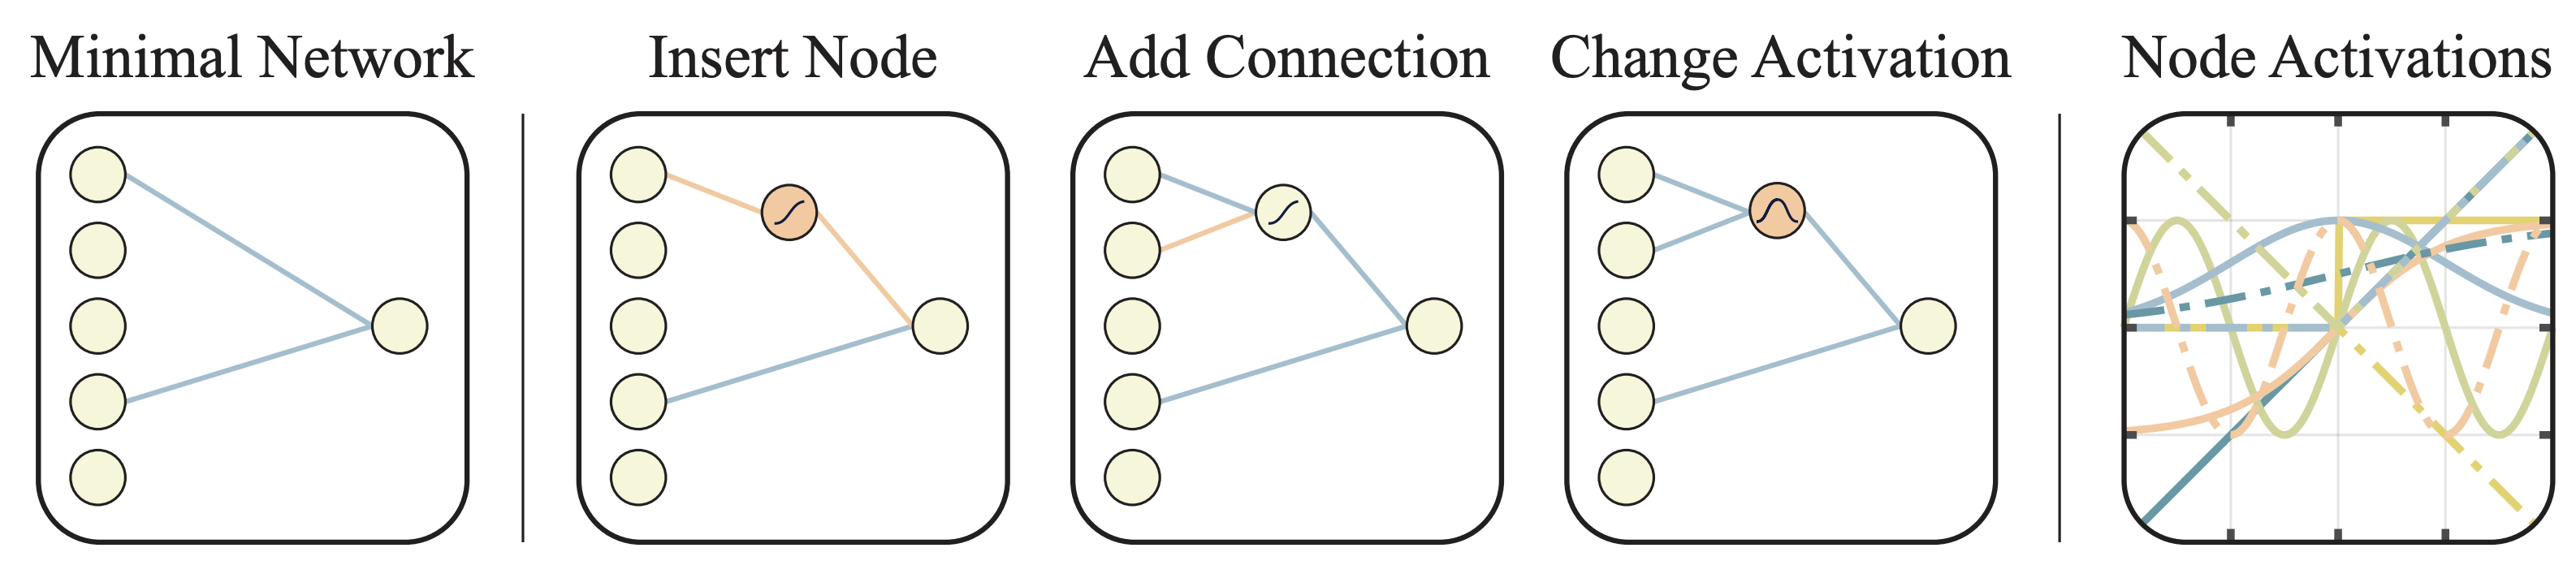
\includegraphics[width=0.7\textwidth]{images/wann-possible-mutations.png}
\end{figure}

\begin{itemize}
    \item\pause Authors use 3 operations to mutate a model: add a connection, add a node, change an activation.
    \item\pause They use $\approx 10$ different activation functions: linear, step, ReLU, sin, cos, etc.
    \item\pause Why don't they have any delete operations?
\end{itemize}
\end{frame}


\begin{frame}{Performance on RL tasks}
They compare their approach against simple agents with hand-crafted architectures trained with policy gradient:
%\begin{itemize}
%    \item\pause  and obtain performance much higher than random
%    \item\pause They also tried to use independent (i.e. not shared) random weights for their architecture
%    \item\pause They also tried to tune shared or non-shared weights to see peak performance of an architecture. 
%\end{itemize}

\begin{figure}
    \centering
    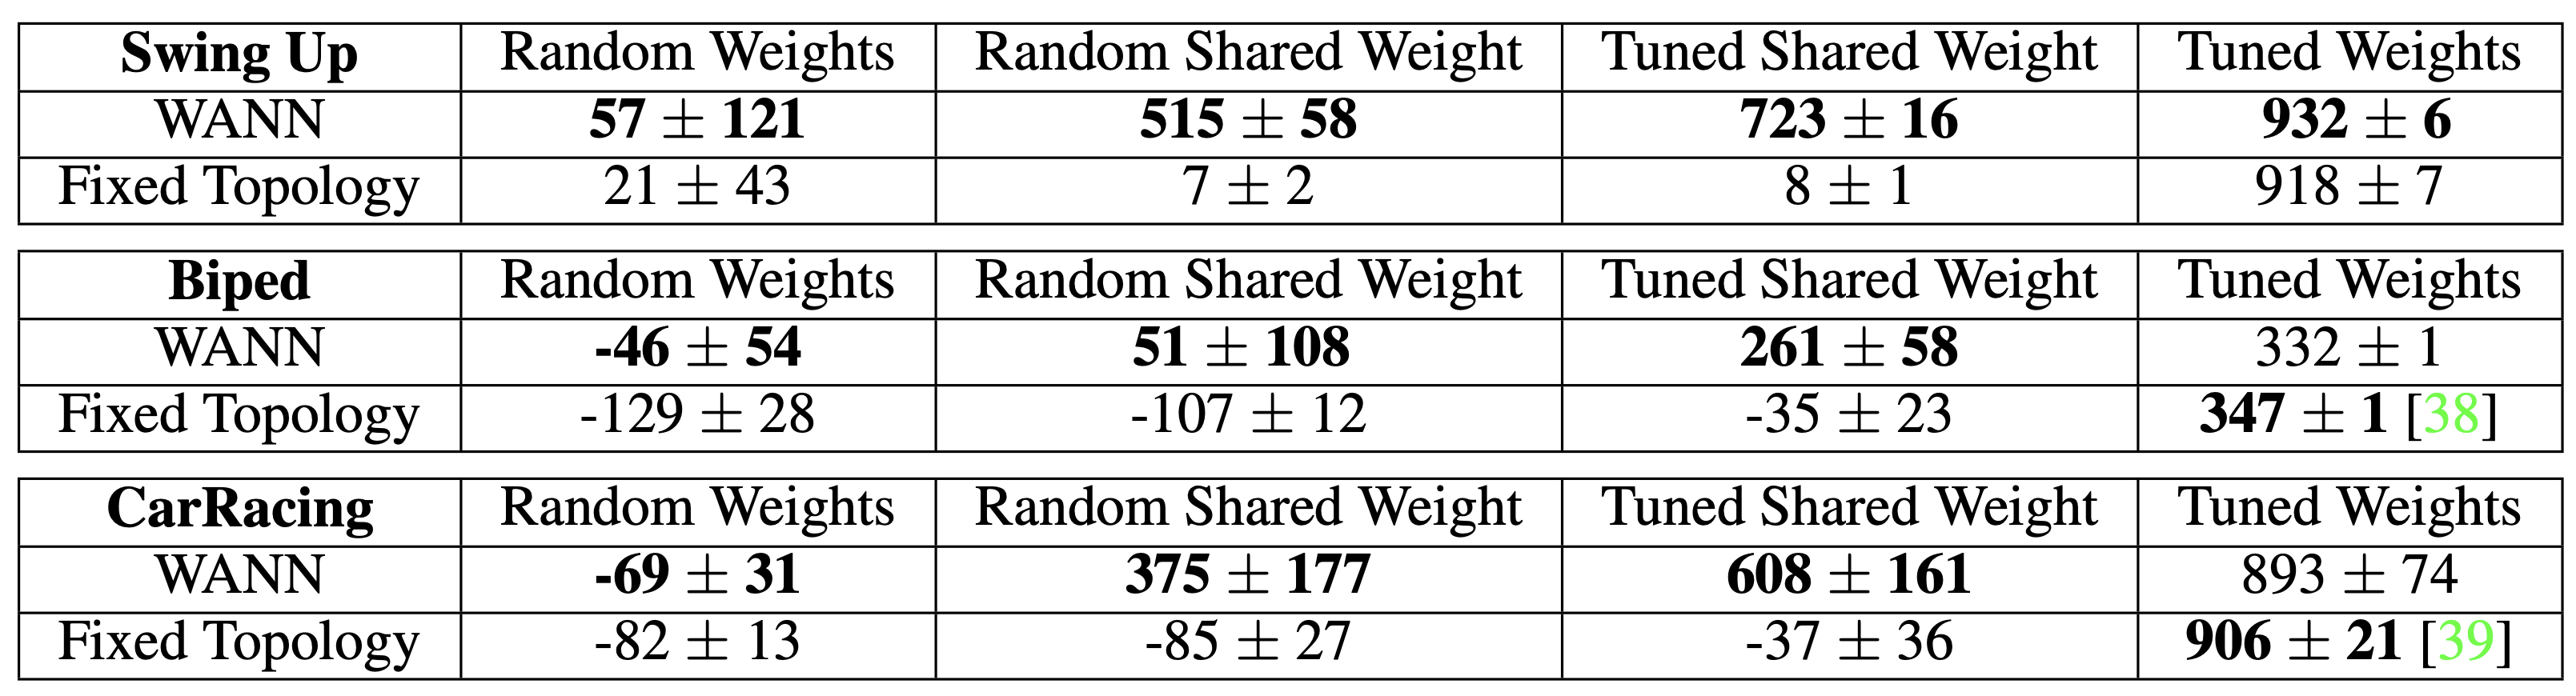
\includegraphics[width=\textwidth]{images/rl-results.png}
\end{figure}

\begin{itemize}
    \item \textit{Random weights}: individual weights drawn from $U(-2, 2)$
    \item \textit{Random shared weight}: a single shared weight drawn from $U(-2, 2)$;
    \item \textit{Tuned shared weight}: the highest performing shared weight value in range $(-2, 2)$;
    \item \textit{Tuned weights}: individual weights tuned using population-based REINFORCE
\end{itemize}
\end{frame}


\begin{frame}{Visualizing best networks for RL tasks}
    \begin{figure}
        \centering
        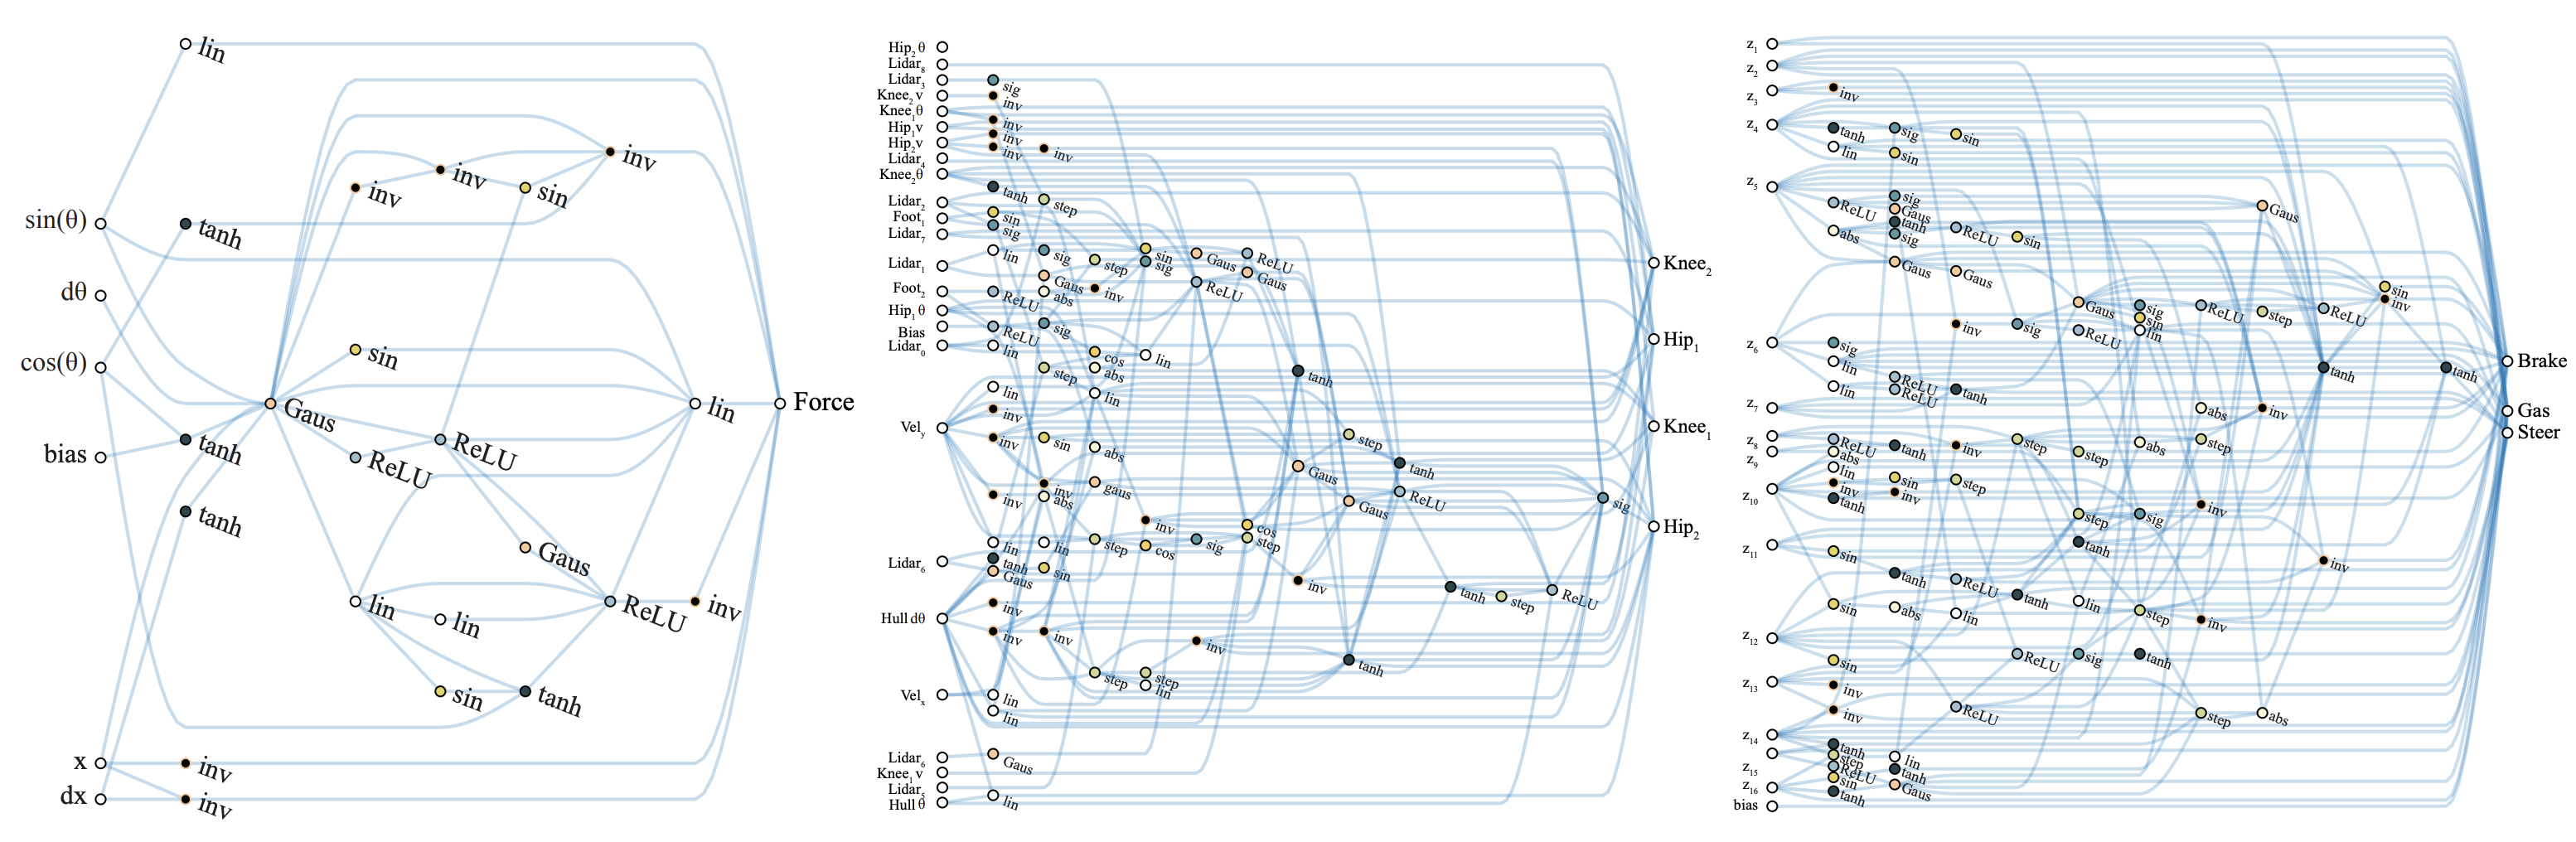
\includegraphics[width=\textwidth]{images/champion-networks-for-cc-tasks.png}
    \end{figure}
\end{frame}


\begin{frame}{MNIST performance}
    \begin{figure}
        \centering
        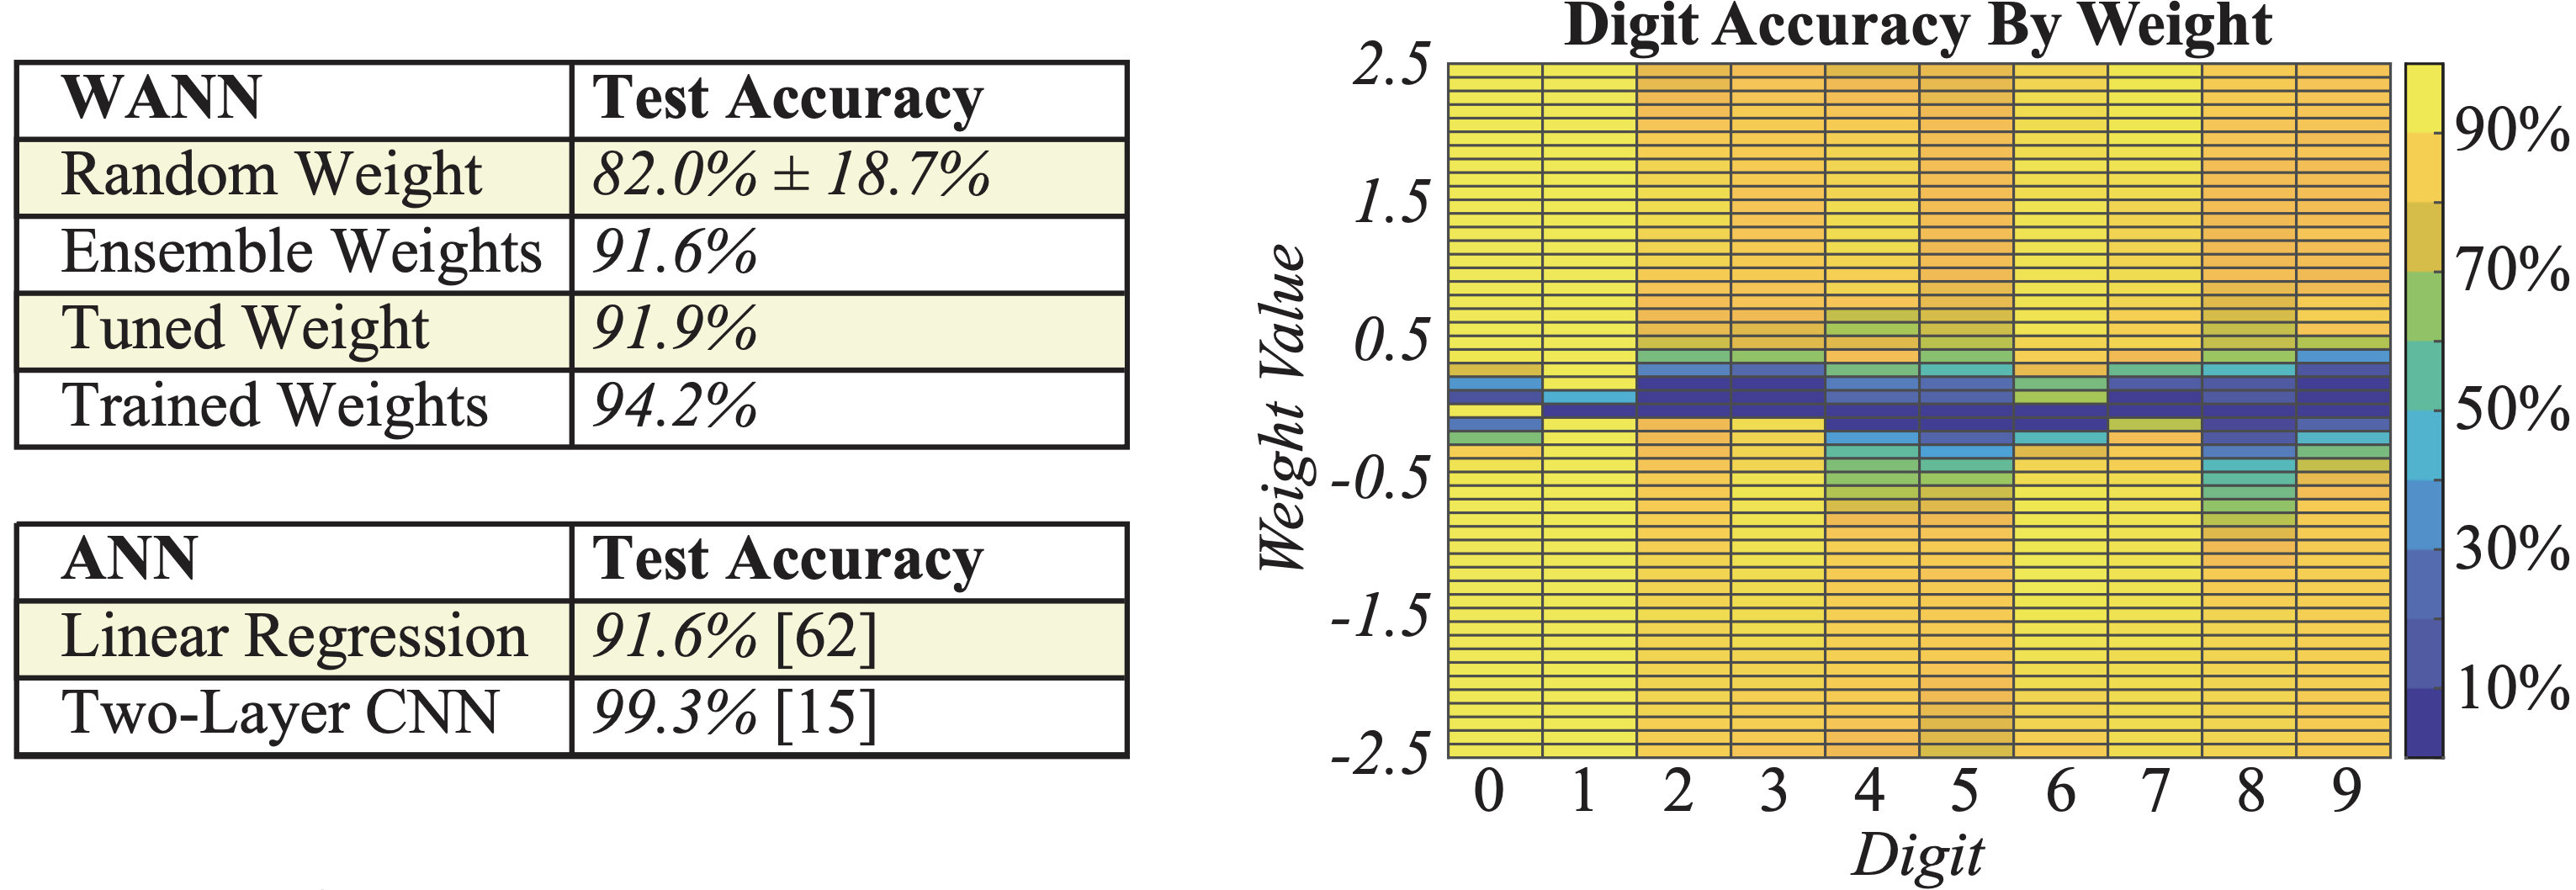
\includegraphics[width=\textwidth]{images/mnist-performance.png}
    \end{figure}
    
    \begin{itemize}
        \item\pause Performance is close to a linear model, but has small amount of weights
        \item\pause Ensembling over different random weights allows to improve the performance
    \end{itemize}
\end{frame}


\begin{frame}{Visualizing the best network for MNIST}
    \begin{figure}
        \centering
        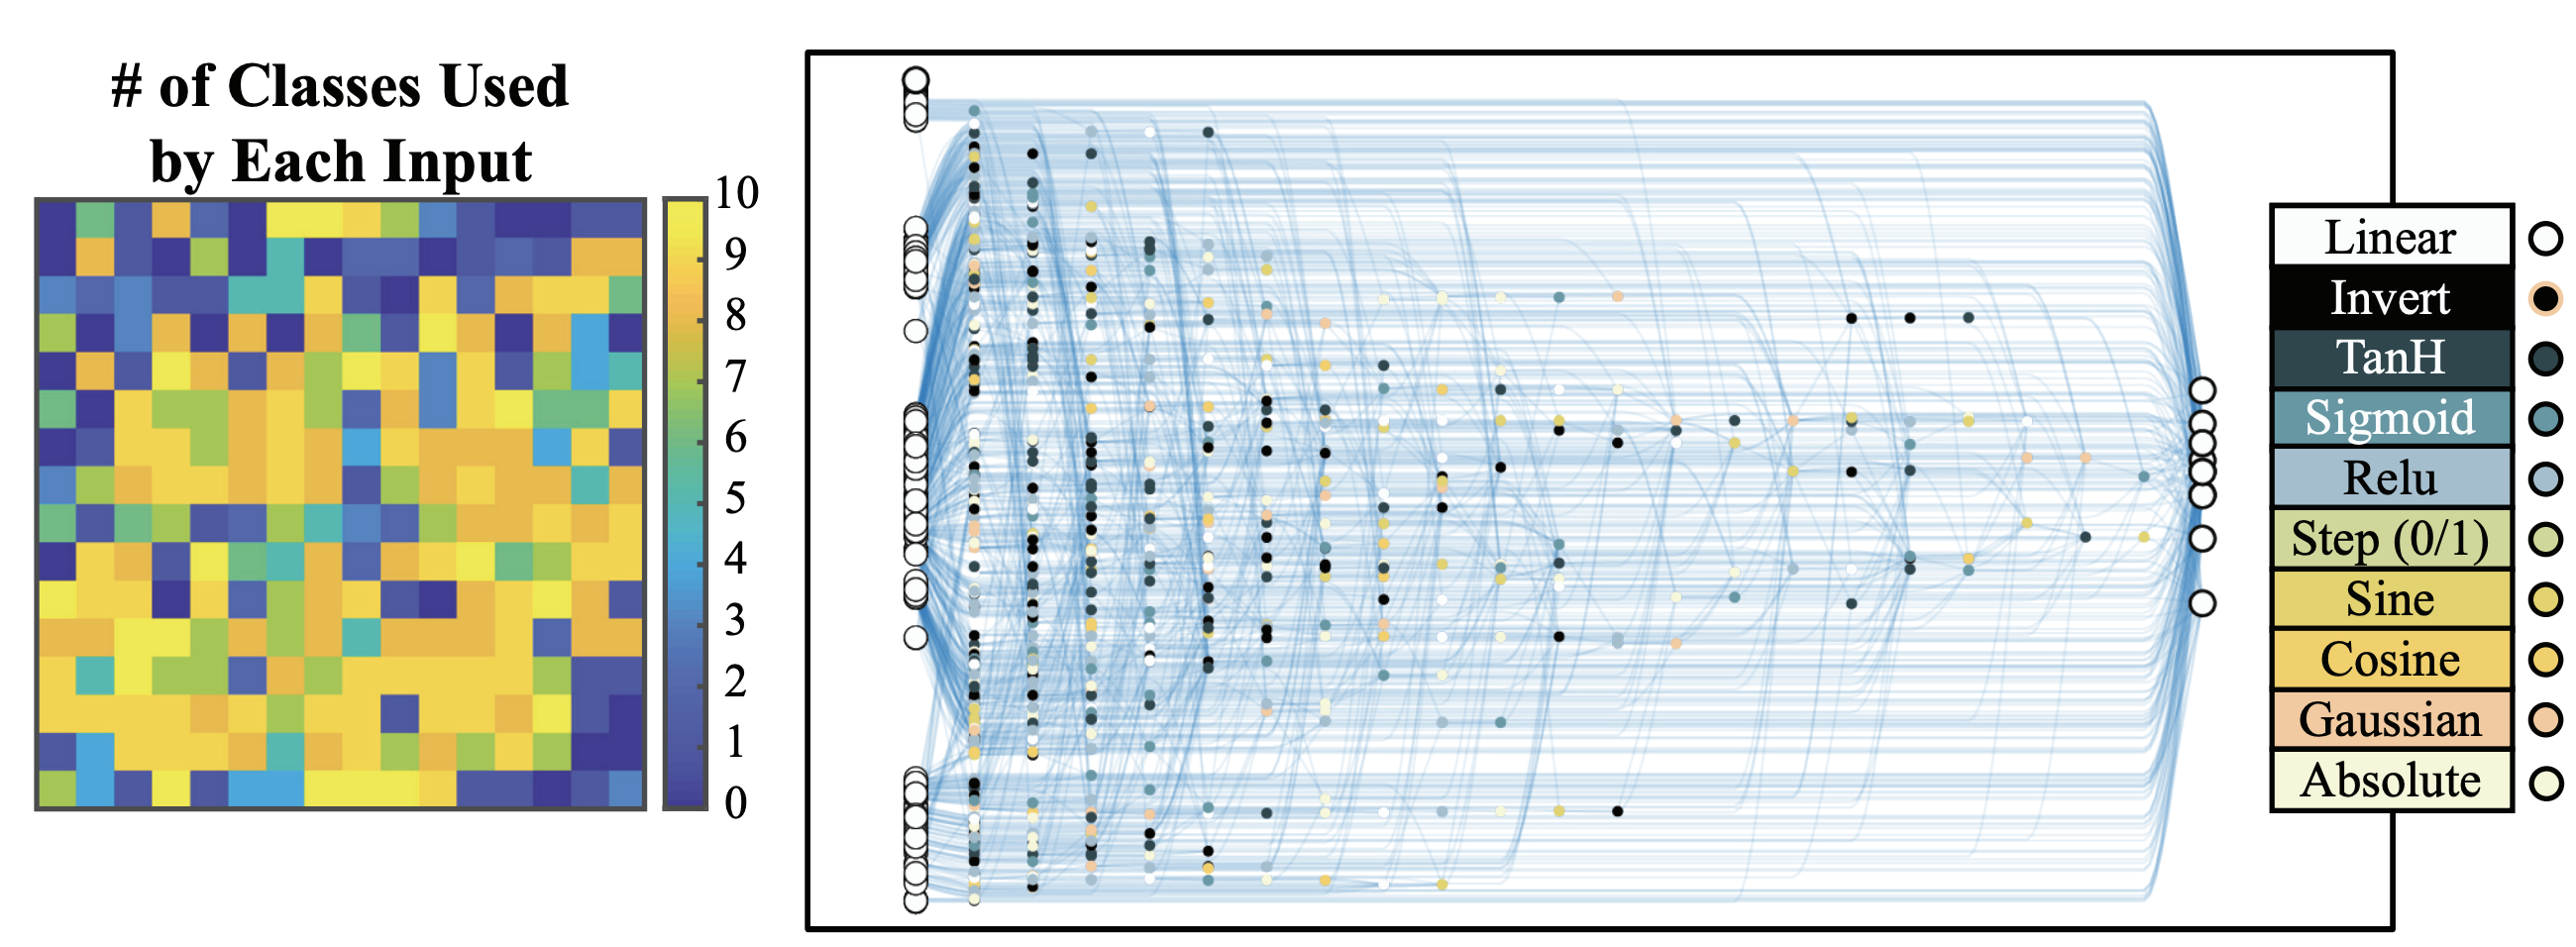
\includegraphics[width=\textwidth]{images/wann-mnist-visualization.png}
    \end{figure}
    From the left figure one can see that different output neurons are connected to different input neurons.
\end{frame}

\begin{frame}{Conclusion}
    \begin{itemize}
        \item An interesting work direction
        \item Resulted architectures with ``true'' random weights (i.e. non-shared) perform much worse.
        \item We do not have much information in the weights, but we have a lot of information in the connectivity pattern.
    \end{itemize}
\end{frame}

\end{document}
